% PrototypeDevelopmentLifecycle.tex
\subsection{Lifecycle}
This section provides an overview of the Prototype Development Lifecycle.

\subsubsection*{Conceptualization and Requirements Definition}
\begin{itemize}
  \item The prototype must have four photodiodes in an xy pattern with respective circuitry required to output ~0-5 Volts that will be read by an Arduino based Data Acquisition System (DAQ). The circuit must be able to react to light intensity changes, however the change will be at low frequency ( below 1Hz) as a satellite attitude is considered to change only gradually.
  \item While the prototype may not have a high accuracy, it is hoped that it will be enough to measure light position changes roughly, even if at a low accuracy of ~10° or ~20° but this will remain to be seen.  
  \item The prototype within the scope of this paper will show the ability to detect the position of light at normal room conditions, therefore it does not need to withstand temperature changes or radiation that a final product would require if deployed in space.
  \item Interface requirements: the prototype electrical output needs to be compatible with the Arduino Analog to Digital Converter (ADC) input. Therefore, the signal shall not go below 0 Volts or exeed 5 volts. 
  \item Size and weight are not of high importance, but the device must fit in the testing equipment, which is the Renewable Energy Demonstrator arch. Preferably a height not higher than 5cm.
\end{itemize}
%%%%%%%%%%%%rewritten up to here ^&&&&&&&&&&&&&&&&& move this line lower when done
\subsubsection*{Theoretical Design}

\paragraph{Photodiodes} were researched and several options were found, most of which were quite expensive, such as 2D PSD type sensors like the Hamamatsu S5990 but were both prohibitivly expensive and Surface Mount Device style (SMD), which would have been harder to prototype but would allow for much higher resolutions, while also complicating the project. A decision was made to base the project on 1D photodiodes, and four Hamamatsu S5971 were purchased, which offered a good compromise in price and specifications: for under £10 a piece, the S5971 has the following specifications:

\begin{table}[h]
  \centering
  \caption{S5971 Photodiode Specifications}
  \begin{tabular}{|l|c|}
  \hline
  \textbf{Parameter} & \textbf{Value} \\
  \hline
  Spectral response range ($\lambda$) & 320 to 1060 nm \\
  \hline
  Peak sensitivity wavelength ($\lambda_p$) & 920 nm \\
  \hline
  Photosensitivity S (A/W) at $\lambda_p$ & 0.64 \\
  \hline
  Photosensitivity S (A/W) at 780 nm & 0.55 \\
  \hline
  Photosensitivity S (A/W) at 830 nm & 0.6 \\
  \hline
  Short circuit current Isc & 1.0 $\mu$A \\
  \hline
  Dark current Id (Typical) & 0.07 nA$^{*3}$ \\
  \hline
  Dark current Id (Maximum) & 1 nA$^{*3}$ \\
  \hline
  Cutoff frequency fc & 0.1 GHz$^{*3}$ \\
  \hline
  Terminal capacitance Ct (f=1 MHz) & 3 pF$^{*3}$ \\
  \hline
  Noise equivalent power NEP ($V_R$=10 V, $\lambda$=$\lambda_p$) & 7.4 $\times$ 10$^{-15}$ W/Hz$^{1/2}$ \\
  \hline
  \end{tabular}
  \begin{tablenotes}
  \small
  \item[*3] $V_R$ = 10 V
  \end{tablenotes}
  \end{table}

Although the higher versions such as S5972-3 have better specifications, such as frequency cutoff of 1GHz and lower Dark current, these were not needed for our project, higher frequency cut off not needed due the static nature of the light source and dark current, while it could affect a case where one of the diodes is fully in the dark, a voltage offeset would be noticeable, but with a voltage resolution restricted by the Arduino DAQ to 4.88mV/step, it was deemed acceptable:
\begin{equation} \label{eq:darkCurrentOffset}
  \begin{split}
V_\text{offset-TIA} &= I_d \times R_f \\
&= 0.07 \text{ nA} \times 1 \text{ M}\Omega \\
&= 70 \text{ }\mu\text{V}
  \end{split}
\end{equation}
\addequation{DC Offset Voltage at TIA Output Due to Dark Current}
\begin{equation} \label{eq:totalDCoffset}
  \begin{split}
V_\text{offset-total} &= V_\text{offset-TIA} \times \text{Gain}_\text{post-amp} \\
&= 70 \text{ }\mu\text{V} \times 16 \\
&= 1.12 \text{ mV}
  \end{split}
\end{equation}
\addequation{Total DC Offset After Post-Amplification}
Equation \ref{eq:totalDCoffset} above shows the final dark current would be a maximum of 1.12mV which is below what the ADC can detect. 

\paragraph{Sun Sensor Geometry and Aperture Design} was decided to be in a T shape, providing an x-y layout with two photodiodes in the x direction and two photodiodes in the y direction. Combined with an aperture design that covers one half of each diode, as represented in Figure \ref{fig:diodeApertureDiagram}.

% Photodiode Aperture Diagram
%
\begin{figure}[htbp] %h-ere t-op b-ottom p-page (separte) -good to allow all htbp to give the compiler more options
    \centering
    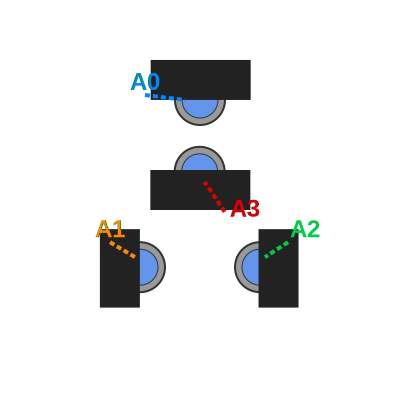
\includegraphics[width=0.6\textwidth]{chapters/methodology/prototype/diodeApertureDiagram.png}
    \caption{Rough Diagram of Photodiode Array with Apertures}
    \label{fig:diodeApertureDiagram}
\end{figure}


\begin{itemize}
  \item Develop mathematical models for sun vector determination
  \item Simulate sensor performance under various lighting conditions
\end{itemize}

\subsubsection*{Preliminary Design}
\begin{itemize}
  \item The design of the Prototype must have four photodiodes in an xy patern with respective apertures placed such that they cover opposite halfs of the photodides. This is to facilitate light location detection by the aperture shadowing the photodiode when the light is on one side but not the other.
\end{itemize}

\subsubsection*{Component Selection and Procurement}
\begin{itemize}
  \item Select appropriate photodiodes (spectral response, sensitivity)
  \item Choose microcontroller/processor
  \item Source analog-to-digital converters
  \item Identify appropriate materials for aperture and housing
  \item Procure test equipment for validation
\end{itemize}

\subsubsection*{Breadboard Testing}
\begin{itemize}
  \item Assemble basic circuit on breadboard
  \item Test photodiode response characteristics
  \item Verify analog front-end performance
  \item Validate signal processing approach
  \item Identify design weaknesses and optimization opportunities
\end{itemize}

\subsubsection*{First Prototype Development}
\begin{itemize}
  \item Design printed circuit board (PCB)
  \item Manufacture PCB
  \item Design and fabricate aperture mask
  \item Develop housing/enclosure
  \item Assemble prototype components
  \item Write initial firmware implementation
\end{itemize}

\subsubsection*{Initial Testing and Characterization}
\begin{itemize}
  \item Conduct functional testing
  \item Measure photodiode response curves
  \item Characterize sun angle determination accuracy
  \item Test temperature sensitivity
  \item Evaluate power consumption
  \item Assess signal-to-noise ratio
\end{itemize}

\subsubsection*{Design Refinement}
\begin{itemize}
  \item Analyze test results
  \item Modify aperture design if needed
  \item Optimize photodiode configuration
  \item Update signal processing algorithms
  \item Refine PCB layout
  \item Improve firmware algorithms
\end{itemize}

\subsubsection*{Second Prototype Development}
\begin{itemize}
  \item Implement design improvements
  \item Manufacture revised PCB
  \item Fabricate improved aperture
  \item Enhance housing design
  \item Update firmware with optimized algorithms
  \item Assemble refined prototype
\end{itemize}

\subsubsection*{Comprehensive Testing}
\begin{itemize}
  \item Laboratory performance testing (angular accuracy, resolution)
  \item Environmental testing (thermal cycling, vibration)
  \item Radiation testing (if applicable for space applications)
  \item Interface compatibility testing
  \item Long-term stability assessment
\end{itemize}

\subsubsection*{Validation and Calibration}
\begin{itemize}
  \item Develop calibration procedures
  \item Create calibration fixtures
  \item Perform sensor calibration
  \item Document calibration coefficients
  \item Validate sensor performance against requirements
\end{itemize}

\subsubsection*{Documentation and Production Readiness}
\begin{itemize}
  \item Create detailed technical specifications
  \item Document calibration procedures
  \item Prepare assembly instructions
  \item Write user manual/interface control document
  \item Develop acceptance test procedures
\end{itemize}

\subsubsection*{Pre-production Prototype}
\begin{itemize}
  \item Build small batch of pre-production units
  \item Conduct acceptance testing
  \item Verify production processes
  \item Validate consistency between units
  \item Finalize design for production
\end{itemize}

\subsubsection*{Technology Transfer to Production}
\begin{itemize}
  \item Document manufacturing processes
  \item Train production personnel
  \item Establish quality control procedures
  \item Define production testing requirements
  \item Prepare for volume manufacturing
\end{itemize}


